\begin{frame}
  \frametitle{Wave mixing}
  \begin{center}
  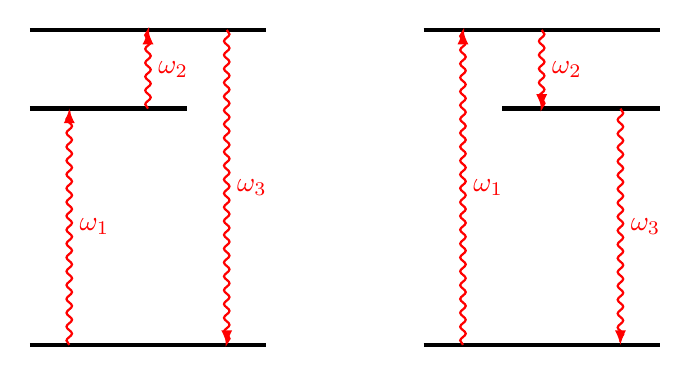
\begin{tikzpicture}[
    ph/.style={
      -latex,
      decorate,
      decoration={snake,amplitude=1,segment length=5pt},
      red,
      thick
    },
    lvl/.style={
      ultra thick
    },
    %scale=0.8,
    ]

    \begin{scope}
      \draw[lvl] (0,0) -- +(3,0);
      \draw[lvl] (0,3) -- +(2,0);
      \draw[lvl] (0,4) -- +(3,0);
      \draw[ph] (.5,0) -- +(0,3) node[midway,right] {$\omega_1$};
      \draw[ph] (1.5,3) -- +(0,1) node[midway,right] {$\omega_2$};

      \draw[lvl] (2,0) -- +(1,0);
      \draw[lvl] (2,4) -- +(1,0);
      \draw[ph] (2.5,4) -- +(0,-4) node[midway,right] {$\omega_3$};
    \end{scope}

    \begin{scope}[xshift=5cm]
      \draw[lvl] (0,0) -- +(3,0);
      \draw[lvl] (0,4) -- +(3,0);
      \draw[lvl] (1,3) -- +(2,0);

      \draw[ph] (0.5,0) -- +(0,4) node[midway,right] {$\omega_1$};
      \draw[ph] (1.5,4) -- +(0,-1) node[midway,right] {$\omega_2$};
      \draw[ph] (2.5,3) -- +(0,-3) node[midway,right] {$\omega_3$};
    \end{scope}
  \end{tikzpicture}
  \end{center}
\end{frame}

%%% Local Variables: 
%%% mode: latex
%%% TeX-master: "nonlinearslides"
%%% End: 
